\chapter{Tree}

\section{Binary Tree}
\subsection{Basic Operations}
\runinhead{Get parent ref.} To get a parent reference (implicitly), \textit{return the Node} of the current recursion function to its parent to maintain the path. Sample code:
\begin{java}
Node deleteMin(Node x) {
    if (x.left == null) return x.right;
    x.left = deleteMin(x.left);
    // x.count = 1+size(x.left)+size(x.right);
    return x;
}
\end{java}
\runinhead{Construct path from root to target.} To search a node in binary tree (not necessarily BST), use dfs:
\begin{python}
def dfs(self, root, t, path, found):
    # post-call check
    if not root: return        
    if found[0]: return 

    path.append(root)
    if root == t:
        found[0] = True

    self.dfs(root.left, t, path, found)
    self.dfs(root.right, t, path, found)
    if not found[0]:
        path.pop()  # 1 pop() corresponds to 1 append()
\end{python}
The \pyinline{found} is a wrapper for boolean to keep it referenced by all calling stack. 

\runinhead{Lowest common ancestor.} In BST, the searching is straightforward. In normal binary tree, construct the path from root to $node_1$ and $node_2$ respectively, and \textbf{diff} the two paths. Time complexity: $O(\lg n)$, space complexity: $O(\lg n)$. 

If the parent pointer is provided, it is possible to reduce the space complexity to $O(1)$, by using two pointers: 
\begin{python}
def find_LCA(n1, n2):
    if not n1 or not n2:
        return None 
        
    d1, d2 = depth(n1), depth(n2)
    if d2 < d1:
        n1, n2 = n2, n1
        d1, d2 = d2, d1
        
    # move to the same depth 
    for _ in xrange(d2-d1):
        n2 = n2.parent  

    while n1 and not n1 == n2:  
        n1 = n1.parent
        n2 = n2.parent
        
    return n1
\end{python}

\runinhead{Find all paths.} Find all paths from root to leafs. For every currently visiting node, add itself to path; search left, search right and pop itself. Record current result when reaching the leaf.
\begin{python}
def dfs_path(self, cur, path, ret):
    if not cur: return

    path.append(cur)
    if not cur.left and not cur.right:
        ret.append("->".join(map(repr, path)))

    self.dfs_path(cur.left, path, ret)
    self.dfs_path(cur.right, path, ret)
    path.pop()
\end{python}

\runinhead{Leftmost node.} Find the leftmost node. 
\begin{python}
def leftmost(self, cur, l):
    """
    :param l: offset from center 0, negative means left side. 
    """
    if not cur: return l
    return min(self.leftmost(cur.left, l-1), 
               self.leftmost(cur.right, l+1))
\end{python}

Rightmost node can be similarly found.

\runinhead{Diameter of a tree.} The diameter of a tree $\equiv$ longest path in the tree.

Core clues:
\begin{enumerate}
\item Start from any vertex, bfs to reach the farthest leaf.
\item Start from this leaf node, bfs to reach the other farthest leaf. 
\end{enumerate}
\begin{python}
_, _, last = self.bfs(0, V)
level, pi, last = self.bfs(last, V)
\end{python}

\subsection{Morris Traversal} 
Traversal with O(1) space. \footnote{\href{http://www.cnblogs.com/AnnieKim/archive/2013/06/15/MorrisTraversal.html}{ref}}

Time complexity $O(3n).$ - find \pyinline{pre} twice, \pyinline{cur} traverse once. \begin{figure}[hbtp]
\centering
\subfloat{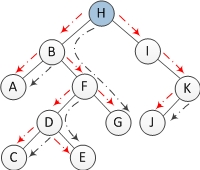
\includegraphics[height=1.2in]{morris_time}}
\caption{Morris traversal time complexity}
\label{fig:morrisTime}
\end{figure}

\subsubsection{Inoder}
Assign the current node's in-order predecessor's right child to itself (threading). Two ptr \pyinline{cur}, \pyinline{pre}. 

Process:
\begin{enumerate}
\item If no left, \textit{consume} \pyinline{cur}, go right 
\item If left, find in-order predecessor \pyinline{pre}
\begin{enumerate}
\item If no thread (i.e. no \pyinline{pre} right child), assign it to \pyinline{cur}; go left
\item If thread, \textit{consume} \pyinline{cur}, go right. ($\equiv$ no left). 
\end{enumerate}
\end{enumerate}

\begin{figure*}[hbtp]
\centering
\subfloat{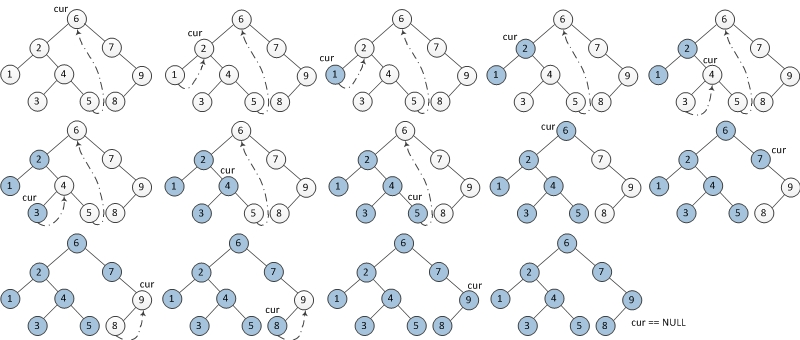
\includegraphics[height=2.4in]{morris_inorder}}
\caption{Morris inorder traversal}
\label{fig:morrisInorder}
\end{figure*}

Code:
\begin{python}
def morris_inorder(self, root):
    cur = root
    while cur:
        if not cur.left:
            self.consume(cur)
            cur = cur.right
        else:
            pre = cur.left
            while pre.right and pre.right != cur:
                pre = pre.right

            if not pre.right:
                pre.right = cur
                cur = cur.left
            else:
                pre.right = None
                self.consume(cur)
                cur = cur.right
\end{python}
\subsubsection{Preoder}
Similar to inorder. 

Process:
\begin{enumerate}
\item If no left, \textit{consume} \pyinline{cur}, go right 
\item If left, find in-order predecessor \pyinline{pre}
\begin{enumerate}
\item If no thread (i.e. no \pyinline{pre} right child), assign it to \pyinline{cur}; \textit{consume} \pyinline{cur}, go left
\item If thread, go right. ($\equiv$ no left, but no \textit{consume}, since consume before). 
\end{enumerate}
\end{enumerate}

\subsubsection{Postorder}
More tedious but solvable.
Process:
\begin{enumerate}
\item set a temporary var \pyinline{dump = cur}
\item if no left child, go right
\item if left child, find the in-order predecessor in left tree
\begin{enumerate}
\item if predecessor has no right, set \pyinline{right = cur}, and then goes \pyinline{cur} left
\item if predecessor \pyinline{right == cur}, set \pyinline{right = None}, \textit{reverse} output the path \pyinline{cur.left} to successor, and then goes \pyinline{cur}'s right. 
\end{enumerate}
\end{enumerate}
\begin{figure*}[hbtp]
\centering
\subfloat{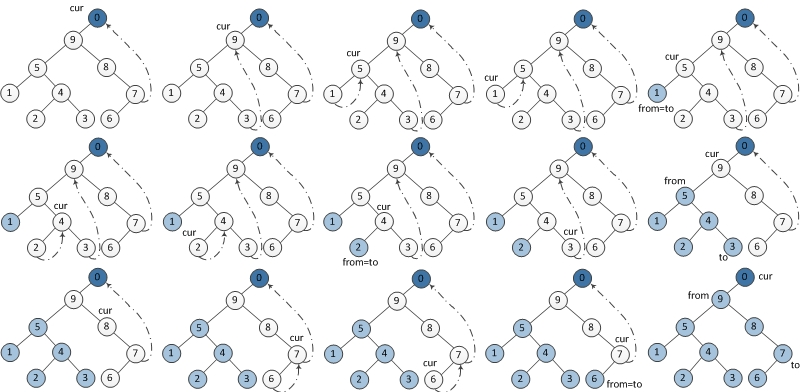
\includegraphics[height=2.8in]{morris_postorder}}
\caption{Morris postorder traversal}
\label{fig:morrisInorder}
\end{figure*}

TODO

\section{Binary Search Tree (BST)}
\runinhead{Array and BST.}Given either the \textbf{preorder} or \textbf{postorder} (but not inorder) traversal of a BST containing N distinct keys, it is possible to reconstruct the shape of the BST. 
\subsection{Rank}
\runinhead{Calculates rank.}
\begin{enumerate}
\item When inserting: 
  \begin{enumerate}
  \item insert to an existing node: \pyinline{node.cnt_this += 1}
  \item insert to left subtree: \pyinline{node.cnt_left += 1}
  \item insert to right subtree: do nothing. 
\end{enumerate}
\item When querying rank:
  \begin{enumerate}
  \item query equals current node: \pyinline{return node.cnt_left}
  \item query goes to \textbf{left} node: \pyinline{return rank(node.left, val)};
  \item query goes to \textbf{right} node: \pyinline{return node.cnt_left} \pyinline{+ node.cnt_this + rank(node.right, val)}
  \end{enumerate}
Notice that the \pyinline{rank} calculates a val's rank in a subtree.
\end{enumerate}

\runinhead{Count of smaller number before itself.} Given an array $A$. For each element $A_i$ in the array, count the number of element before this element $A_i$ is smaller than it and return count number array. Average $O(n \log n)$
\\
Clues:
\begin{enumerate}
\item Put $A[:i+1]$ into a BST; so as to count the rank of $A[i]$ in the BST
\end{enumerate}
Codes:
\begin{python}
class Node(object):
  def __init__(self, val):
    """Records the left subtree size"""
    self.val = val
    self.cnt_left = 0
    self.cnt_this = 0
    self.left, self.right = None, None


class BST(object):
  def __init__(self):
    self.root = None

  def insert(self, root, val):
    """
    :return: subtree's root after insertion
    """
    if not root:
      root = Node(val)

    if root.val == val:
      root.cnt_this += 1
    elif val < root.val:
      root.cnt_left += 1
      root.left = self.insert(root.left, val)
    else:
      root.right = self.insert(root.right, val)

    return root

  def rank(self, root, val):
    """
    Rank in the root's subtree
    :return: number of items smaller than val
    """
    if not root:
      return 0
    if root.val < val:
      return (root.cnt_this+root.cnt_left+
              self.rank(root.right, val))
    elif root.val == val:
      return root.cnt_left
    else:
      return self.rank(root.left, val)


class Solution(object):
  def countOfSmallerNumberII(self, A):
    tree = BST()
    ret = []
    for a in A:
      tree.root = tree.insert(tree.root, a)
      ret.append(tree.rank(tree.root, a))

    return ret
\end{python}
Notice: if worst case $O(n \log n)$ is required, need to use Red-Back Tree - Section \ref{rbtree}. However, there is a more elegant way using Segment Tree - Section \ref{segmentTreeInversionCount}.


\subsection{Range search}
\runinhead{1-d range count}
\begin{java}
int size(Key lo, Key hi) {
    if (contains(hi)) return rank(hi)-rank(lo)+1;
    else              return rank(hi)-rank(lo);
}
\end{java}

\runinhead{Closest value} Find the value in BST that is closet to the \pyinline{target}.
\\
Clues:
\begin{enumerate}
\item Find the value just $\leq$ the target.
\item Find the value just $\geq$ the target.
\end{enumerate}
\
\\
Code for finding either the lower value or higher value:
\begin{python}
def find(self, root, target, ret, lower=True):
  """ret: result container"""
  if not root: return

  if root.val == target:
    ret[0] = root.val
    return

  if root.val < target:
    if lower:
      ret[0] = max(ret[0], root.val)

    self.find(root.right, target, ret, lower)
  else:
    if not lower:
      ret[0] = min(ret[0], root.val)

    self.find(root.left, target, ret, lower)
\end{python}

\runinhead{Closet values} Find $k$ values in BST that are closet to the \pyinline{target}.
\\\\
Clues:
\begin{enumerate}
\item Find the predecessors $\triangleq \{node | node.value \leq target\}$. Store in the stack. 
\item Find the successors $\triangleq \{node | node.value \geq target\}$. Store in the stack.
\item Merge the predecessors and successors as in merge in MergeSort to get the $k$ values. 
\end{enumerate}
\
\\
Code for finding the predecessors:
\begin{python}
def predecessors(self, root, target, stk):
  if not root: return

  self.predecessors(root.left, target, stk)
  if root.val <= target:
    stk.append(root.val)
    self.predecessors(root.right, target, stk)
\end{python}


\section{Binary Index Tree (BIT)}\label{BIT}
\subsection{Introduction}
Compared to Segment Tree \ref{section:segmentTree}, BIT is shorter and more elegant. BIT can do most of things that Segment Tree can do and it is easier to code. BIT updates and queries $$i\rightarrow prefixSum$$ in $O(\log n)$ time; however, Segment Tree can but BIT cannot query $$prefixSum \rightarrow i$$
\subsection{Implementation}
Given an array $A$ of length $n $ starting from $1$. prefix sum $s[i]\triangleq A_1+...+A_i$. BIT uses binary to maintain the array of prefix sum for querying and updating. For $i$-th node in the BIT, 
$$
N[i]=A_{j+1}+...+A_i
$$
, where $j=i-lowbit(i)$, i.e. set $i$'s lowest bit 1 to 0. $lowbit(i)$ can be defined as \pyinline{return i & -i}, using 2's complement. Notice that the summation ends with $A_i$ since easier to \pyinline{set}.

For the range, we use $(j, i]$ here instead of $[j, i)$ since more elegant for \pyinline{get(i)} and \pyinline{set(i)}
\\\\
Clues:
\begin{enumerate}
\item Binary 
\item Low bit
\item BIT uses array index starting from \textbf{1}, because 0 doesn't have $lowbit$. 0 is the dummy root.
\end{enumerate}
\begin{figure}[hbtp]
\centering
\subfloat{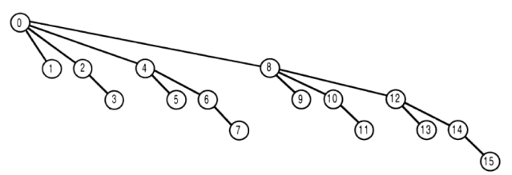
\includegraphics[height=1.1in]{BITget}}
\caption{Binary Indexed Tree \textit{get} Operation}
\label{fig:LABEL}
\end{figure}

\begin{figure}[hbtp]
\centering
\subfloat{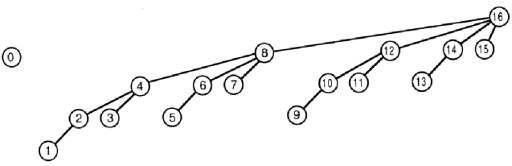
\includegraphics[height=1.05in]{BIT}}
\caption{Binary Indexed Tree \textit{set} Operation}
\label{fig:LABEL}
\end{figure}

Time complexity, longest update is along the leftmost branch, which takes $O(\log_2 n)$ (e.g. 1, 10, 100, 1000, 10000); longest query is along a branch starting with node with all 1's (e.g. 1111, 1110, 1100, 1000), which also takes $O(\log_2 n)$.
\newpage
Code:
\begin{python}
class BIT(object):
    def __init__(self, n):
        """
        BIT uses index starting from 1
        0 is the dummy root 
        """
        self.N = [0 for _ in xrange(n+1)]

    def lowbit(self, i):
        return i & -i

    def get(self, i):
        ret = 0
        while i > 0:
            ret += self.N[i]
            i -= self.lowbit(i)

        return ret
        
    def set(self, i, val):
        while i < len(self.N):
            self.N[i] += val
            i += self.lowbit(i)
\end{python}


\section{Segment Tree}\label{section:segmentTree}
\subsection{Introduction}
Segment Tree is specially built for \textit{range queries}. 

The structure of Segment Tree is a binary tree which each node has two attributes start and end denote an segment/interval. 

Notice that by practice, the interval is normally $[start, end)$ but sometimes it can be $[start, end]$, which depends on the question definition. 

Structure:  
\begin{lstlisting}[columns=flexible]
# a Count Segment Tree
                     [0, 4, count=3]
                     /             \
          [0,2,count=1]             [2,4,count=2]
          /         \               /            \
   [0,1,count=1] [1,2,count=0] [2,3,count=1], [3,4,count=1]
\end{lstlisting}
Variants:
\begin{enumerate}
\item Sum Segment Tree.
\item Min/Max Segment Tree.
\item Count Segment Tree. 
\end{enumerate}

For a Maximum Segment Tree, which each node has an extra value max to store the maximum value in this node's interval.

\subsection{Operations}
Segment Tree does a decent job for range queries.
\\
Components in Segment Tree operations:
\begin{enumerate}
\item Build
\item Query 
\item Modify
\item Search 
\end{enumerate}
Notice:
\begin{enumerate}
\item Only build need to change the start and end recursively.
\item Pre-check is preferred in recursive calls.
\end{enumerate}
Code: Notice the code has abstracted out segment tree functions of sum, min/max or count, by abstracting the subtree combine function to \pyinline{lambda}.
\begin{python}
DEFAULT = 0
f = lambda x, y: x+y


class Node(object):
    def __init__(self, start, end, m):
        self.lo, self.hi, self.m = lo, hi, m
        self.left, self.right = None, None


class SegmentTree(object):
    def __init__(self, A):
        self.A = A
        self.root = self.build_tree(0, len(self.A))

    def build_tree(self, lo, hi):
        """
        segment: [lo, hi)
        Either check lo==hi-1 or have root.right 
        only if have root.left
        """
        if lo >= hi:   return None
        if lo == hi-1: return Node(lo, hi, self.A[lo])

        left  = self.build_tree(lo, (lo+hi)/2)
        right = self.build_tree((lo+hi)/2, hi)

        val = DEFAULT
        if left:  val = f(val, left.m)
        if right: val = f(val, right.m)
        root = Node(lo, hi, val)
        root.left  = left
        root.right = right

        return root

    def query(self, root, lo, hi):
        """
        :type root: Node
        """
        if not root:
            return DEFAULT

        if lo <= root.lo and hi >= root.hi:
            return root.m

        if lo >= root.hi or  hi <= root.hi:
            return DEFAULT

        l = self.query(root.left,  lo, hi)
        r = self.query(root.right, lo, hi)
        return f(l, r)

    def modify(self, root, idx, val):
        """
        :type root: Node
        """
        if not root or idx < root.lo or idx >= root.hi:
            return

        if idx == root.lo and idx == root.hi-1:
            root.m = val
            self.A[idx] = val
            return

        self.modify(root.left,  idx, val)
        self.modify(root.right, idx, val)

        val = DEFAULT
        if root.left:  val = f(val, root.left.m)
        if root.right: val = f(val, root.right.m)
        
        root.m = val
\end{python}
The above code abstracts out segment tree function using \pyinline{lambda}. For a concrete example, see Count Segment Tree \ref{inversionReconstruct}. 

\newpage
\section{Trie}
\subsection{Basic}
Trie is aka radix tree, prefix tree. 
\begin{figure}[hbtp]
\centering
\subfloat{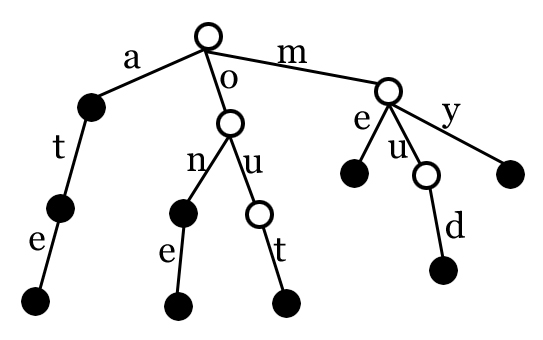
\includegraphics[scale=.30]{trie.jpg}}
\caption{Trie}
\label{fig:trie} 
\end{figure}
\runinhead{Notice:}
\begin{enumerate}
\item Children are stored in HashMap rather than ArrayList. 
\item self.word to stores the word and indicates whether a word ends at the current
node. 
\end{enumerate}
Codes:
\begin{python}
class TrieNode(object):
    def __init__(self, char):
        self.char = char
        self.word = None
        self.children = {}  # map from char to TrieNode


class Trie(object):
    def __init__(self):
        self.root = TrieNode(None)

    def add(self, word):
        word = word.lower()
        cur = self.root
        for c in word:
            if c not in cur.children:
                cur.children[c] = TrieNode(c)
            cur = cur.children[c]
        cur.word = word
\end{python}

\subsection{Advanced}
Implicit storage of word in TrieNode: 
\begin{enumerate}
\item Implicitly stores the current word. 
\item Implicitly stores the current char. 
\item When insert new word, do not override the existing TrieNode. A flag to indicate
whether there is a word ending here.
\end{enumerate}
\newpage
Code:
\begin{python}
class TrieNode:
    def __init__(self):
        """Implicit storage"""
        self.ended = False
        self.children = {}


class Trie:
    def __init__(self):
        self.root = TrieNode()

    def insert(self, word):
        cur = self.root
        for w in word:
            if w not in cur.children:   # not override
                cur.children[w] = TrieNode()
            cur = cur.children[w]

        cur.ended = True

    def search(self, word):
        cur = self.root
        for w in word:
            if w in cur.children:
                cur = cur.children[w]
            else:
                return False

        if not cur.ended:  # not ended here
            return False

        return True

    def startsWith(self, prefix):
        cur = self.root
        for w in prefix:
            if w in cur.children:
                cur = cur.children[w]
            else:
                return False

        return True
\end{python}
\subsection{Applications}
\begin{enumerate}
\item Word search in matrix.
\item Word look up in dictionary.
\end{enumerate}
        
     
